\documentclass[fleqn,xcolor={usenames,dvipsnames},notes,aspectratio=169]{beamer} % [notes=only]
\usepackage{amsmath} % {amssymb,amsfonts}

\usepackage{array,adjustbox} % url

\usepackage{pifont,marvosym} % \ding
% \usepackage{multimedia}
% \usepackage[normalem]{ulem}
% \usepackage{framed,color,ragged2e}
% \usepackage[absolute,overlay]{textpos}
% \definecolor{shadecolor}{rgb}{0.8,0.8,0.8}

\usetheme{boxes}
\setbeamertemplate{navigation symbols}{}
\usepackage{xcolor}
\usepackage{tikz}
\usetikzlibrary{shapes,arrows}
\usetikzlibrary{tikzmark,positioning}
\usetikzlibrary{calc}

\newtheorem*{rawnamedtheorem}{\therawnamedtheorem}
\newcommand{\therawnamedtheorem}{\error}
\newenvironment{namedtheorem}[1]{\renewcommand{\therawnamedtheorem}{#1}
   \begin{rawnamedtheorem}}
  {\end{rawnamedtheorem}}


\title{Paying for privacy preserving messaging}
% \subtitle{Technologies to secure the future Internet}

\author[Burdges \& Kiel]{Jeff Burdges \hspace*{15pt} \and Robert Kiel}
\institute{
  \hspace*{5pt}
  
\includegraphics[scale=0.25]{logos/web3logo.jpg}. % web 3 foundation
  \hspace*{10pt}
  
\includegraphics[scale=0.055]{logos/web3logo.jpg}. % validity labs
}
\date{27.12.2017}

\newcolumntype{R}[2]{%
    >{\adjustbox{angle=#1,lap=\width-(#2)}\bgroup}%
    l%
    <{\egroup}%
}
\newcommand*\rot{\multicolumn{1}{R{45}{1em}}}% no optional argument here, please!

\def\signed #1 (#2){{\leavevmode\unskip\nobreak\hfil\penalty50\hskip2em
  \hbox{}\nobreak\hfil\normalfont --#1 (#2)%
  \parfillskip=0pt \finalhyphendemerits=0 \endgraf}}
% https://tex.stackexchange.com/questions/13756/quote-environment-with-reference-at-the-end-right

\begin{document}


% \begin{frame}
% \begin{center}
% \includegraphics[page=1,scale=0.45]{pics/kohls/dfg_visit.pdf} % trim=0 200 0 0,clip
% \end{center}
% \end{frame}


{\setbeamertemplate{footline}{}
\begin{frame}
\titlepage
\end{frame}
}
% \note{Hello, happy to be here, etc.}
\setcounter{framenumber}{0}


\begin{frame}
\begin{center}
\begin{quote}
``Encryption works. % ''
Properly implemented strong crypto systems are one of the few things that you can rely on.'' \\
% Unfortunately, endpoint security is so terrifically weak that NSA can frequently find ways around it.''
\signed Edward Snowden (2013)
\end{quote}
\end{center}
\end{frame}


% \begin{frame}
% \includegraphics[page=2,scale=0.40,trim=0 0 0 0,clip]{pics/nsa/nsa_v_otr.pdf}
% \end{frame}


\note{
“Encryption works”.  In fact encryption is basically free, provided you hire cryptographers and do the UI properly 

In recent years, we’ve seen enormous progress in making end-to-end encrypted communications practical and user friendly. Signal demonstrated user-friendly end-to-end encrypted messaging and WhatsApp brought it to over a billion users. 

Some snake oil like Telegram remains. There remain serious vulnerabilities either due to poor UI design, like Riot, or else due to trusting phone numbers. And PGP still exists. But overall the story looks good.
}
% Slide with logos of Signal, Wire, etc. perhaps?


\begin{frame}
\begin{columns}[T]
\column{0.55\textwidth}
\bigskip\bigskip
{\it ``We kill people based on metadata''} \\ % \normalfont 
--Michael Hayden (Ex-NSA Director)
% NSA Director `99-`05 and CIA Director `06-`09
\column{0.45\textwidth}
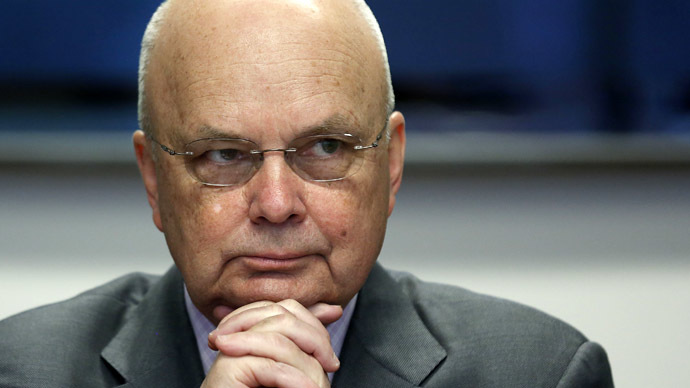
\includegraphics[scale=0.3]{pics/nsa/micheal_hayden-0.jpeg}
\end{columns}
\end{frame}


\note{
We'll speak about metadata protection which cannot be protected by encryption alone.

There are many things referred to as metadata, but we'll speak primarily about netwrok level metadata obtained from monitoring packets and used to answer questions like:
“Who communicates with whom”
“How often does a specific party communicate with another party”
“When does that party sends usually messages to other parties”

We know the government signals intelligence agencies like the NSA primarily collect metadata, and largely on innocent people, thanks to numerous whistleblowers including Mr Snowden.  We also know these agencies are given wide range to interpret this very circumspect data however they like, sometimes blowing up weddings. 
}
% Whats's the difference between Michael Hayden and the Years of Lead guy


\begin{frame}{Who needs their metadata protected?}

Everyone  ;)

\bigskip

Journalists communicating with sources % is the classical answer. 

\bigskip

Potential targets of spear-phishing, kidnapping, etc.
% Zooko talks about crypto-currency enthusiasts' personal security

\bigskip\bigskip % \pause

Financial networks were already adversarial anyways..

\end{frame}


\note{Who needs their metadata protected? % And under what threat model?

Journalists communicating with sources is the classical answer. 

Zooko Wilcox loves this example of crypto-currency enthusiasts
fearing for their safety because they live in or travel to
South american countries with a kidnapping problem. 
% This is not so remote:  In the early 1970s, Carla Bruni's
% family moved to France to escape the Years of Lead in Italy.

As a rule, financial networks are adversarial,
 and distributed ones even more so,
so anonymity is simply a that we need for mechanism design, to prevent front running, etc.

WhatsApp..
}
% Of course Facebook buying WhatsApp for \$19 B and nixing
% WhatsApp's perfectly reasonable \$1 per year payment scheme says 
% that users still pay in data, but now just metadata.


\begin{frame}{How valuable is metadata?}

``At the time of the sale [to Facebook], WhatsApp was profitable with fee revenue, although it is unclear by how much''
% https://twitter.com/FredericJacobs/status/1004757759269658624

\bigskip

\begin{itemize}
\item[2012] WhatsApp adds encryption 
\item[2014] Facebook pays 19 billion USD for WhatsApp
\item[2016] Facebook added encryption to Messanger \\
            WhatsApp drops \$1 per year fee
\end{itemize}

\end{frame}


\note{Facebook is overcharging for WhatsApp by >> \$1 per year}


% \begin{frame}{}
%   \begin{center}
%     Time to resist traffic analysis!
% \includegraphics[trim=0 20 0 0,clip,width=0.5\textwidth]{pics/white_rabbit}
% \end{center}
% \end{frame}


% \begin{frame}{}
%   \vfill
%   {\bf Existing solutions?}
% 
%   \vfill
%   \begin{center}
%     \includegraphics[width=0.6\textwidth]{pics/tor/tor_logo}
%   \end{center}
% \end{frame}


\begin{frame}
Six years ago the NSA considered Tor effective, \\
\hspace*{3pt} at least against mass location tracking.

\begin{center}
\includegraphics[page=2,scale=0.35,trim=0 200 0 0,clip]{pics/tor/nsa-tor-stinks.pdf}
\end{center}
\end{frame}


\note{Tor is good}


\begin{frame}
\begin{center}
  {\bf Tor is not enough}
\end{center}

\vfill

% \begin{quote}
{\it ``[Tor does not] protect against an attacker who can see .. both traffic going into [and] coming out of the Tor network .. % } 
as simple statistics let you decide whether [both flows] match up.''}
\\ \ \hfil \normalfont --Roger Dingledine, ``One cell is enough ..''
% \end{quote}
% https://blog.torproject.org/one-cell-enough-break-tors-anonymity

\vfill

See: \\
% Aaron Johnson, Chris Wacek, Rob Jansen, Micah Scherr, and Paul Syverson.
\hspace*{3pt} Johnson, Wacek, Jansen, Scherr, Syverson.  {\it Users Get Routed: \\ 
\hspace*{3pt} Traffic Correlation on Tor By Realistic Adversaries.} (CCS 2013)
% \hspace*{3pt} 
\end{frame}
% TODO: Ask Paul Syverson about his upcoming WPES paper on deanonymizing Tor ...


\begin{frame}%{Website Fingerprinting}
You only need one side if the other side behaves predictably, \\
\hspace*{3pt} like a website.. \hspace*{3pt}\only<2>{or a {\em synchronous} DApp} \\
\smallskip

\begin{center}
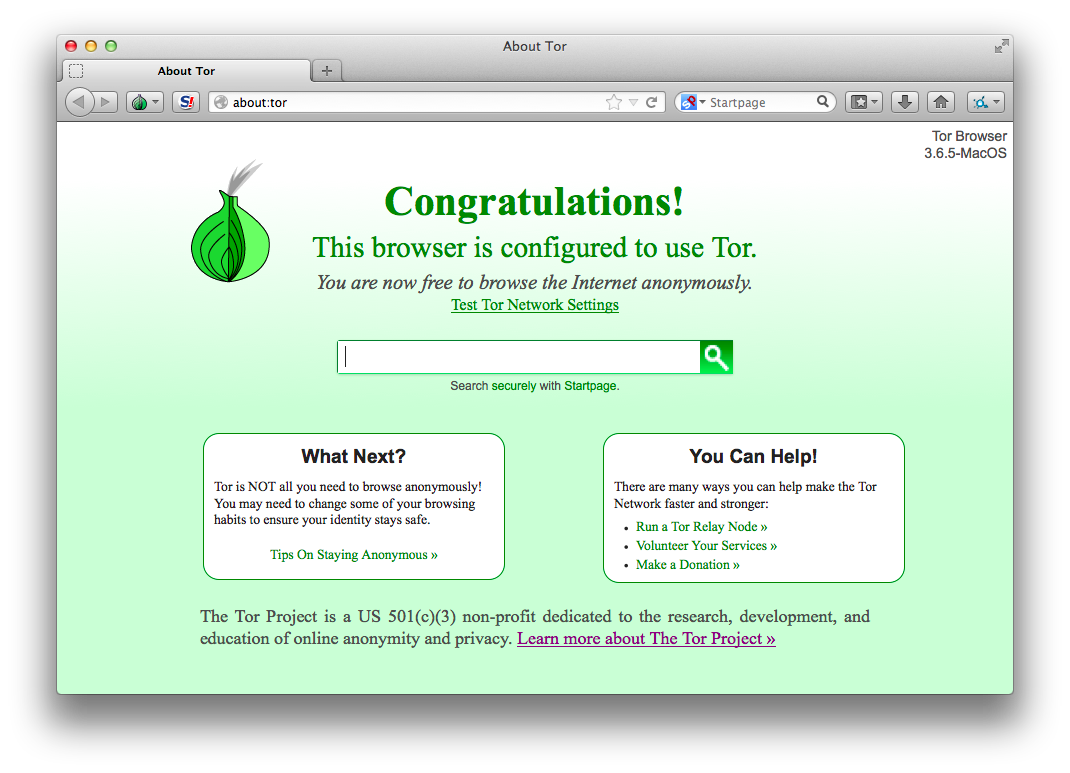
\includegraphics[width=0.6\textwidth]{pics/tor/Tor_screenshot}
\end{center}
\smallskip

Admit defeat on HTTP per se.. \hspace*{3pt}\only<2>{\hspace*{3pt} but not on DApps}
\end{frame}
% ``[INSERT ACADEMIC QUOTE]'' \\
% \ \hfill ---[WHOEVER]


\note{Anonymity folk talk about website fingerprinting, but 
you could easily fingerprint important details of say a distributed
crypto-currency trading too.  

There are messaging programs like Biar and Riccochet that run
over Tor without exposing metadata to any central server, but..

We might not physically travel to sit around the same table, but
we tend to live in the same country as our friends or even use the same ISPs.
}


\begin{frame}

Mix networks are among the oldest anonymity tools, dating back to \\ \medskip

\hspace*{3pt} David Chaum. {\em Untraceable electronic mail, return addresses, and \\
\hspace*{3pt} digital pseudonyms}, Comm. ACM, 24, 2 (Feb. 1981); 84-90

\medskip\bigskip\bigskip

We know other anonymity system designs, like
\begin{itemize}
\item Dining cryptographer's networks (DC-nets)
\item Private Information Retrieval (PIR) 
\end{itemize}
but they all scale poorly.. % \\ \hspace*{1pt}
 most need quadratic bandwidth per user.
\end{frame}

\note{
PIR fits narrower applications and scales poorly.
% Information theoretic classical variant consume bandwidth quadratic
% in the anonymity set, but computational variant merely consume 
% insane computational resources.

JB: DC-nets face numerous challenges, including costs that scale
quadratically in the anonymity set.  If you pay a lot for a small
anonymity set then you anonymity set will consist of people working
together.  A whistle blower does not benefit from hiding which
reporter ho spoke to, while a boss ordering illegal activities does.
Small anonymity sets favor rich criminals.

hybrid DC mix??}


\begin{frame}{What is a mix network?}
\begin{center}
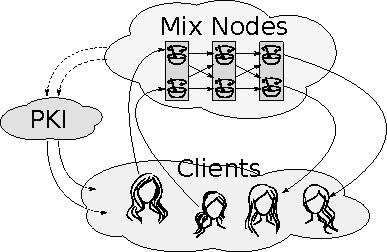
\includegraphics[width=0.8\textwidth]{pics/mix/initial}
\end{center}
\end{frame}


\note{Mix nets resemble Tor superficially, and need many similar features,
like a way for clients to learn about the network.  Mix nets differ from
Tor in that they ``mix'' packets with secret delays, adding latency.}


\begin{frame}{How do you make a mix network?}
\begin{center}
\begin{tabular}{rl}
 Packet format &
  Sphinx by George Danezis and Ian Goldberg \smallskip \\ \smallskip
 PKI &
  Consensus like Tor vs gossip like I2P \\ \smallskip
 Topology &
  Free route vs stratified vs ... \\ \smallskip
 Mix strategy &
  Continuous time : Poison, Stop-n-Go, etc. \\ \smallskip
 Cover traffic & 
  Loopix by Piotrowska, et al. \\ \smallskip
% & \\ \smallskip
% API & Make devs love latency?? \\ \smallskip
% Apps & Make users love latency?? \\ \smallskip
% Economics & ??? \\
\end{tabular}
\end{center}
\end{frame}


\begin{frame}
\begin{namedtheorem}{Anonymity Trilemma}[Das, Meiser, Mohammadi, Kate (2017)]
Anonymity cannot scale better than $|\mathrm{cover\ traffic}| \cdot |\mathrm{latency}|$
\end{namedtheorem}
% Anonymity scales no better than roughly $|\mathrm{cover\ traffic}| \cdot |\mathrm{latency}|$

\bigskip
\bigskip

% Roger Dingledine answers ideas for adding cover traffic \\ to 
% or by saying they don't know if cover traffic helps.
Tor's situation: \quad $|\mathrm{cover\ traffic}| * 0 = 0$

% \pause
\bigskip
Anonymity cost still looks quadratic.. {\it but not in users.}
% Intuitively, anonymity cost for mix networks looks quadratic too, \\
% \hspace*{3pt} split across bandwidth and latency, but cost is linear in users.

\end{frame}
% https://eprint.iacr.org/2017/954
% Debajyoti Das, Sebastian Meiser, Esfandiar Mohammadi, Aniket Kate.
% {\it Anonymity Trilemma: Strong Anonymity, Low Bandwidth, Low Latency---Choose Two}


\note{JB: Are we done?  Yes kinda.
% Tor's latency is not actually zero
Roger Dingledine answers ideas for adding cover traffic to 
Tor by saying they don't know if cover traffic helps.}


\begin{frame}
% \begin{center}
  \begin{quote}
  ``The universe believes in encryption'' \quad --Julian Assange (2012) % \\
  % \signed Julian Assange (2012)
  \end{quote}
% https://cryptome.org/2012/12/assange-crypto-arms.htm
% \end{center}

\bigskip\bigskip\bigskip

Encryption is free, but you must pay for anonymity.

\pause\bigskip\bigskip\bigskip
\hspace*{60pt} Can we measure contributions?

\end{frame}


\note{JB: Nobody make such religious sounding statements for anonymity.

... in other words you must ask people to do work on your behalf.

If work is being done, then we have an economy of sorts, and we should try to measure contributions.}



\begin{frame}{How do you make a mix network?}
\begin{center}
\begin{tabular}{rl}
 Packet format &
  Sphinx by George Danezis and Ian Goldberg \smallskip \\ \smallskip
 PKI &
  Consensus like Tor vs gossip like I2P \\ \smallskip
 Topology &
  Free route vs stratified vs ... \\ \smallskip
 Mix strategy &
  Continuous time : Poison, Stop-n-Go, etc. \\ \smallskip
 Cover traffic & 
  Loopix by Piotrowska, et al. \\ \smallskip
 & \\ \smallskip
 API & Make devs love latency?? \\ \smallskip
 Apps & Make users love latency?? \\ \smallskip
 Economics & ??? \\
\end{tabular}
\end{center}
\end{frame}



\begin{frame}{Idea 1: Blind signed tokens}

Can users pay mix nodes with blind signed tokens?${}^\dag$

\bigskip

Almost, but double spending protections need either \\
\hspace*{3pt} centralisation or penalties.


\bigskip\bigskip\bigskip

% \hspace*{3pt}
${}^\dag$ David Chaum. {\em Blind Signatures for Untraceable Payments} CRYPTO '82: 199--203

\end{frame}

\note{
David Chaum invented an anonymous payment technology called blind signatures
 about two years before he invented mix networks.

In principle users could pay mix nodes in blind signed tokens, but we'd require double spending protections, meaning either some fast centralised database or else some penalty for double spending.  

We do not like centralised database, so forget that.  We dislike penalties here because they require startup costs paid by users.

As an aside, if we did like larger penalties then we could even use blind certificate schemes like Coconut based on blind signature scheme by Pointcheval and Sanders.

Also, all blind signature schemes require heavier cryptographic schemes like pairings or RSA, or more round trips.}

\begin{frame}{Idea 2a: Direct payment channels}

Can users pay mix nodes through payment channels?

\bigskip\bigskip

Almost all payment channel constructions lack anonymity.. \\ \smallskip
\hspace{3pt}  Also BOLT is too expensive and ...

\bigskip\bigskip

Instead use payment channels that follow the packet's route.

\end{frame}

\note{
Anonymous payment channels like BOLT are complex, heavy, and require zero knowledge chains, like Zcash.

We no longer need anonymous payment channels because we forward money along the same route as the packet.
}

\begin{frame}{Idea 2b: Payment channels along route}
$$ \longrightarrow A \longrightarrow B \longrightarrow C \longrightarrow $$

\begin{itemize}
\item C unlocks payment from A to B, but B makes unlinkable.
\item If a packet is dropped then remaining funds should be burnt.
\item ...
\end{itemize}

\end{frame}

\note{
...

If the user is refunded, then their guard node learns this fact.
If the money stays put, then dropping packets becomes profitable.

Who burns the funds?  Who enforces the burning?  Aka on which channel are the funds burnt?

%If a packet is dropped then remaining funds should be burnt because
%  refunding users deanonymizes them, but
%  if funds stay put then dropping packets becomes profitable.

}


\begin{frame}{Idea 3: Proof-of-onion}

Could ``secret shopper'' packets allocate node rewards fairly?

\bigskip\medskip

Rule \#1.  Do not weaken anonymity. \\ \medskip

Randomly deanonymise very few secret shoppers from cover traffic.

\bigskip

Rule \#2.  Running honest nodes should be the optimal strategy. \\ \medskip

Build cover traffic with a verifiable random function (VRF):
\begin{itemize}
\item Identify lottery players by staking accounts.
\item Each player commits to a VRF key and a network view.
\item Seed VRFs with subsequent collaborative randomness.. \\
 \hspace*{3pt}  And strictly limit VRF evaluations.
\item Construct packet using only VRF output, including \\
 \hspace*{3pt} a Merkle proof of sampling the network view honestly. 
\end{itemize}

\end{frame}


\note{
All nodes send cover traffic in Loopix, but..

We do not require all nodes or all traffic types be eligible for the lottery, as nodes get paid even if they do not send the packet.
}


\end{document}











\begin{frame}{Don't roll your own packet format!} % {Sphinx by George Danezis and Ian Goldberg}
\begin{center}
Sphinx is a remarkably compact and secure packet format \\ % \hspace*{5pt} 
designed by George Danezis and Ian Goldberg.
\bigskip
 
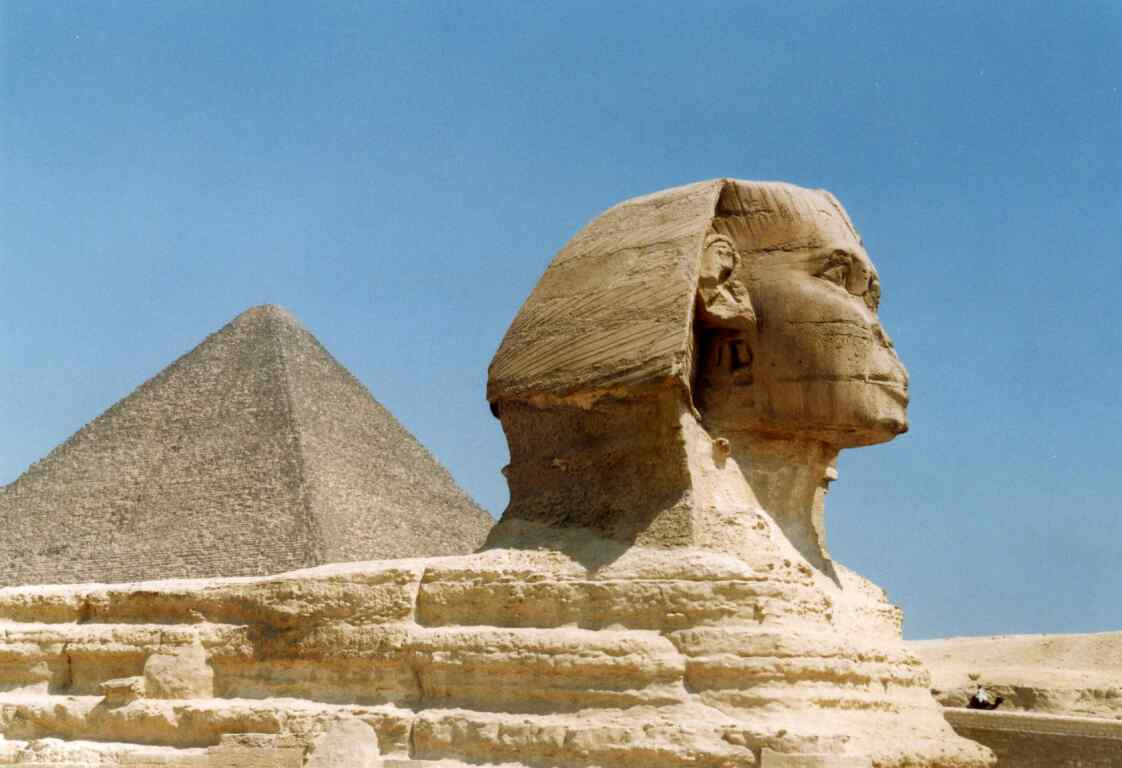
\includegraphics[width=0.7\textwidth]{pics/Sphinx}\tikzmark{sphinx}
\end{center}

Security proof in the universal composability model, \\ % (Canetti 2001)
\hspace*{5pt} using earlier work by Camenisch \& Lysyanskaya 2005.

\begin{tikzpicture}[remember picture,overlay,red]
\node<2-> (h) at (10,5.5) {Header};
\node<2-> (b) at (10,3.5) {Body};
\draw<2-> [->,thick] (h) edge (8,5) (b) edge (8,3);
\end{tikzpicture}
\end{frame}


\note{JB: ..

Anonymity protocols involve more blackmagic than normal cryptographic protocols.

LIONESS.  AEZ by Rogaway.  HHFHFH by DJB, et al. }


\begin{frame} % [t] % {Sphinx packets} 
A Sphinx packet is a tuple $(\alpha,\beta,\gamma,\delta)$ where \\
% \hspace*{4pt}  $\alpha$ is an elliptic curve point, \\
% \hspace*{4pt}  $\beta$ is routing data onion encrypted using a stream cipher, \\
% \hspace*{4pt}  $\gamma$ is a MAC for $\beta$, \\
% give the header, and \\
% \hspace*{4pt}  $\delta$ is the packet body onion encrypted with a wide-block cipher. \\

 \vspace*{-18pt} \[
\left. \begin{array}{@{}rl@{}}
  \alpha & \text{is an elliptic curve point,}\\
  \beta & \text{is routing data onion encrypted with a stream cipher,}\\
  \gamma & \text{is a MAC for $\beta$, and} \\
\end{array} \right\} \text{header}
\] \vspace*{-10pt} \[
\left. \, \begin{array}{@{}rl@{}}
  \delta & \text{is the packet body onion encrypted with a wide-block cipher}.
\end{array} \right.
\] % https://tex.stackexchange.com/questions/240868/how-to-write-cases-with-latex

\bigskip\medskip

\def\svgwidth{\columnwidth}
\input{pics/mix/sphinx.pdf_tex}

% A mix node $n$ processing $(\alpha,\beta,\gamma,\delta)$ obtains the next node $n'$ \\
% and a new packet $(\alpha',\beta',\gamma',\delta')$ to which it is bitwise unlinkable.

\end{frame}









\begin{frame}
\begin{center}
\end{center}
\end{frame}


\begin{frame}
\end{frame}


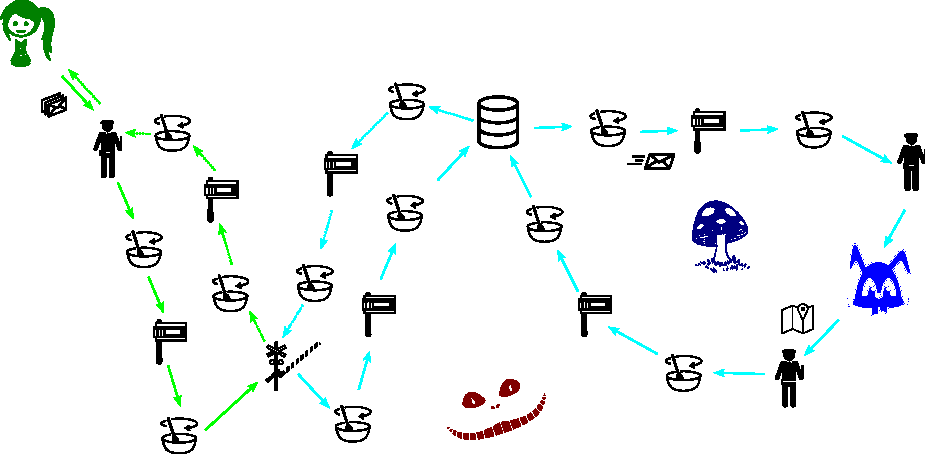
\includegraphics[width=\textwidth]{pics/lake_architecture1}

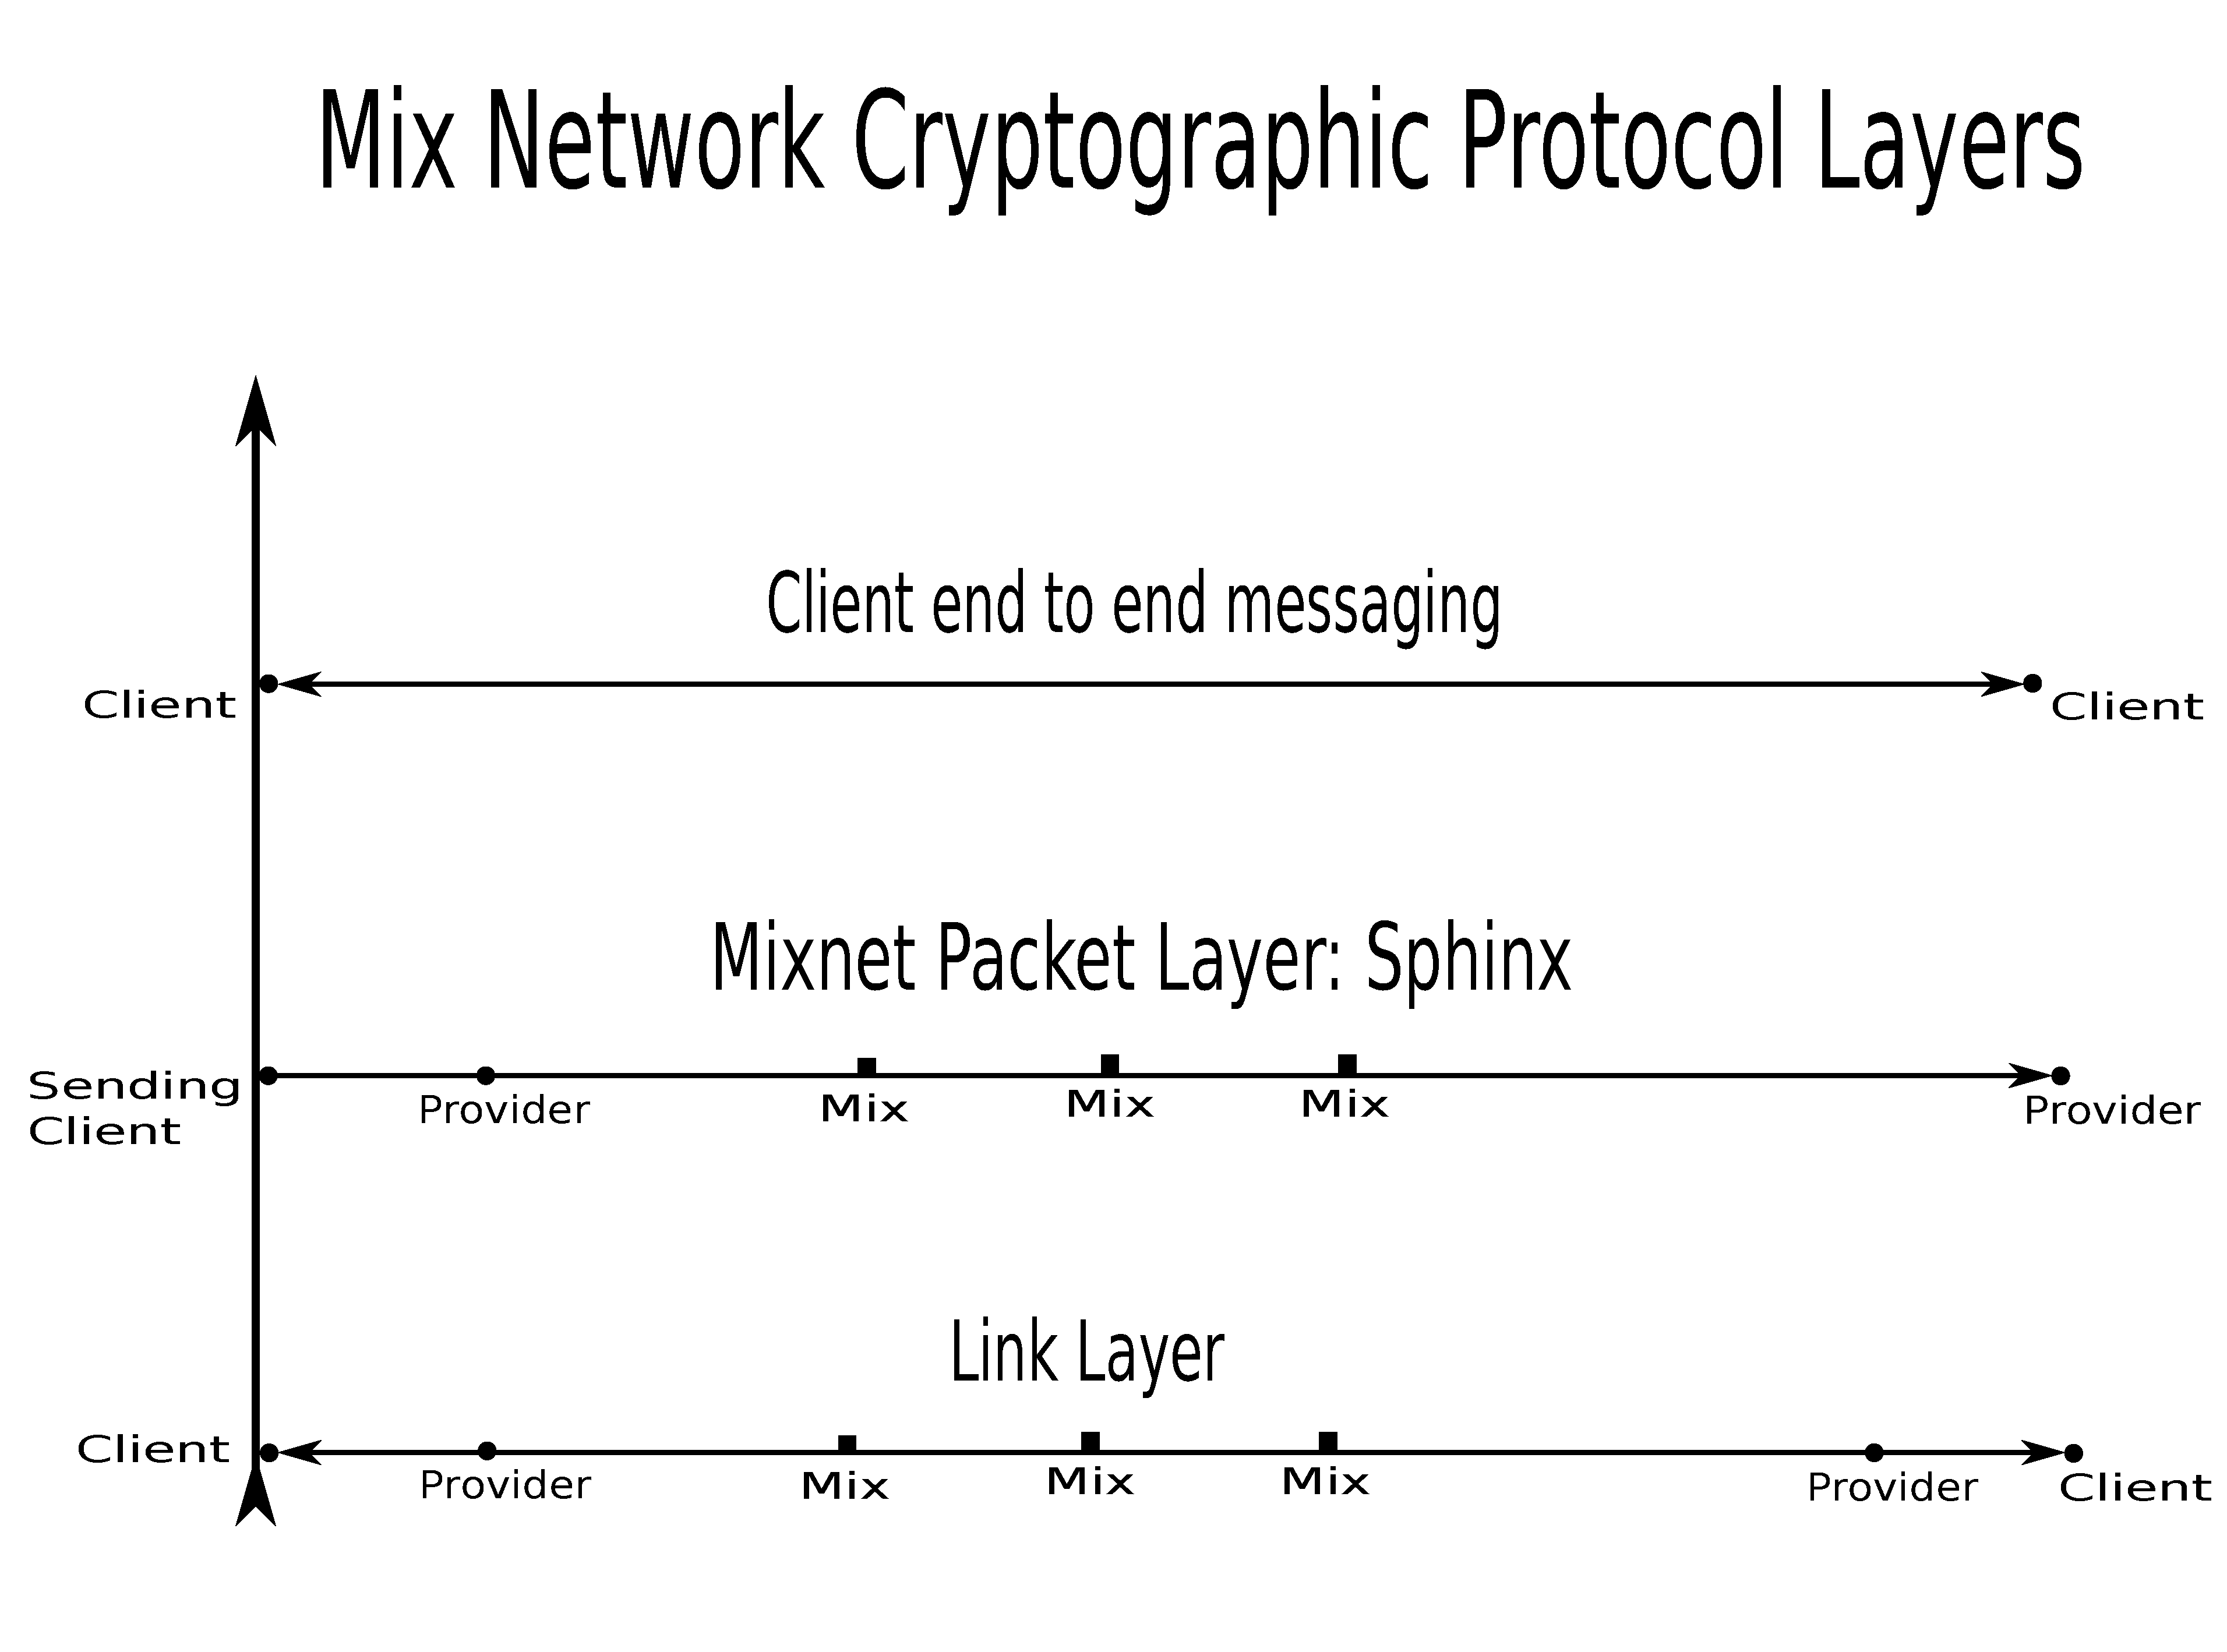
\includegraphics[width=0.8\textwidth]{pics/mixnet_layer_cake}




